% Chapter 14 -- Claim: Selling Options Earns a Reliable Premium
% Requires: amsmath, amssymb, booktabs, array, tabularx, graphicx, tcolorbox (breakable, skins), hyperref or url.
% Defines the callout box only if the preamble has not.
\providecolor{fenavy}{HTML}{1B2A6B}
\providecolor{feshade}{HTML}{F3F5FA}
\makeatletter
\@ifundefined{callout}{%
  \newtcolorbox{callout}{breakable, enhanced,
    colback=white, colframe=gray!70, boxrule=0.5pt, arc=1mm,
    borderline west={2.5pt}{0pt}{gray!70},
    left=8pt, right=8pt, top=4pt, bottom=4pt}%
}{}
\makeatother

\chapter{Claim: Selling Options Earns a Reliable Premium}
\label{ch:14}

An insurance company collects premiums every month and pays out claims now and then. If it prices its policies a little above expected claims, it earns a steady profit, with the occasional very bad year when a hurricane hits. An investor who sells stock-index options is in the same business. A put option is insurance against a market fall. Its seller collects a premium up front and pays out when the market drops.

The claim in this chapter is that this insurance is systematically overpriced: option prices imply more volatility than the market goes on to deliver, so sellers earn a premium. It is one of the best-documented facts in derivatives markets, and it underpins a large industry of option-income funds, covered-call ETFs and volatility-selling strategies.

The question is what kind of premium it is. A reliable premium for bearing a risk that others want to shed is one thing. A strategy that wins small most months and loses large in a few, while carrying most of the stock market's risk, is another. The two can look alike in a backtest, and the evidence has to separate them.

By the end of the chapter you will be able to:

\begin{itemize}
  \item describe call and put payoffs and use put--call parity to show that a covered call and a cash-secured put are the same position;
  \item price an option by Black--Scholes, compute its Greeks, and back out implied volatility;
  \item define the VIX and the variance risk premium, and estimate a seller's expected gain from the gap between implied and realized volatility;
  \item state the claim that selling options earns a reliable premium, and separate the variance risk premium from the returns of option-income strategies;
  \item measure option-strategy performance with beta-matched benchmarks, up and down betas and the manipulation-proof performance measure;
  \item judge what an option-income fund is likely to deliver, and what can go wrong.
\end{itemize}

\section{Foundations: options, Black--Scholes and implied volatility}
\label{sec:14-foundations}

\textbf{Payoffs.} A \textbf{call} gives the right to buy an asset at the \textbf{strike price} $K$ on the expiry date $T$; at expiry it pays $\max(S_T - K, 0)$, where $S_T$ is the asset's price then. A \textbf{put} gives the right to sell; it pays $\max(K - S_T, 0)$. An option is \textbf{at the money} when $K$ equals the current price, \textbf{out of the money} when exercising now would pay nothing (a put with $K$ below $S$), and \textbf{in the money} otherwise. The buyer pays a \textbf{premium}; the seller (or \textbf{writer}) receives it and takes on the obligation.

\textbf{Put--call parity.} For European options, which can be exercised only at expiry, on a non-dividend-paying asset with the same strike and expiry:
\begin{equation}
  C - P = S - K e^{-rT}
  \label{eq:14-parity}
\end{equation}
Rearranged, \emph{stock plus a short call} equals \emph{cash of $Ke^{-rT}$ plus a short put}. A \textbf{covered call} (own the stock, sell a call) and a \textbf{cash-secured put} (hold the strike in bills, sell a put) with the same strike are the same position.

\textbf{Black--Scholes--Merton.} If the stock follows a geometric Brownian motion with constant volatility $\sigma$, an option can be replicated by trading the stock and a bond, so its price does not depend on investors' risk preferences (Black and Scholes 1973; Merton 1973):
\begin{equation}
  C = S\,N(d_1) - K e^{-rT} N(d_2), \qquad P = K e^{-rT} N(-d_2) - S\,N(-d_1)
  \label{eq:14-bs}
\end{equation}
\begin{equation}
  d_1 = \frac{\ln(S/K) + (r + \sigma^2/2)\,T}{\sigma\sqrt{T}}, \qquad d_2 = d_1 - \sigma\sqrt{T}
  \label{eq:14-d}
\end{equation}
where $N$ is the standard normal distribution function. Chapter 15 tests the replication argument itself.

\textbf{The Greeks} measure sensitivities.

\begin{itemize}
  \item \textbf{Delta} ($\partial V/\partial S$) is the number of shares that hedge the option: $N(d_1)$ for a call, $N(d_1) - 1$ for a put.
  \item \textbf{Gamma} is the change in delta as $S$ moves.
  \item \textbf{Vega} is the change in price per unit change in $\sigma$.
  \item \textbf{Theta} is the change in price as time passes.
\end{itemize}

An option seller is short gamma and short vega, and collects theta: time decay works in the seller's favour, large moves against.

\textbf{Implied volatility} is the $\sigma$ that makes the Black--Scholes price equal the market price. It is the market's price of volatility, not a forecast in the statistical sense. \textbf{Realized volatility} is the standard deviation of returns that actually occurs over the option's life. Implied volatility differs across strikes: for stock indexes, out-of-the-money puts trade at higher implied volatilities than at-the-money options, a pattern called the \textbf{skew} (Chapter 15).

\textbf{The VIX} is Cboe's index of 30-day implied volatility for the S\&P 500, computed from a strip of out-of-the-money calls and puts. Its square approximates the fair strike of a 30-day \textbf{variance swap}, a contract that pays the difference between realized variance and a fixed strike. The \textbf{variance risk premium} is the expected difference between implied (risk-neutral) variance and realized variance.

\textbf{Worked example.} The index is at 100, the risk-free rate is 4\%, and a one-month at-the-money put trades at an implied volatility of 20\%.

\begin{itemize}
  \item Black--Scholes price: $P = \$2.14$ per \$100 of index. The call is worth \$2.47; the difference, \$0.33, equals $100 - 100\,e^{-0.04/12}$, as parity requires.
  \item Suppose volatility over the month turns out to be 16\%. At 16\%, the put would have been worth \$1.68. The seller's expected gain is roughly $\$2.14 - \$1.68 = \$0.46$, or vega (\$0.115 per vol point) times the 4-point gap.
  \item That is an \emph{expected} gain. If the index falls 10\% during the month, the put pays \$10 and the seller loses $\$10 - \$2.14 = \$7.86$, about seventeen months of expected gains at \$0.46 a month (Figure~\ref{fig:14-put}).
\end{itemize}

\begin{figure}[htbp]
\centering
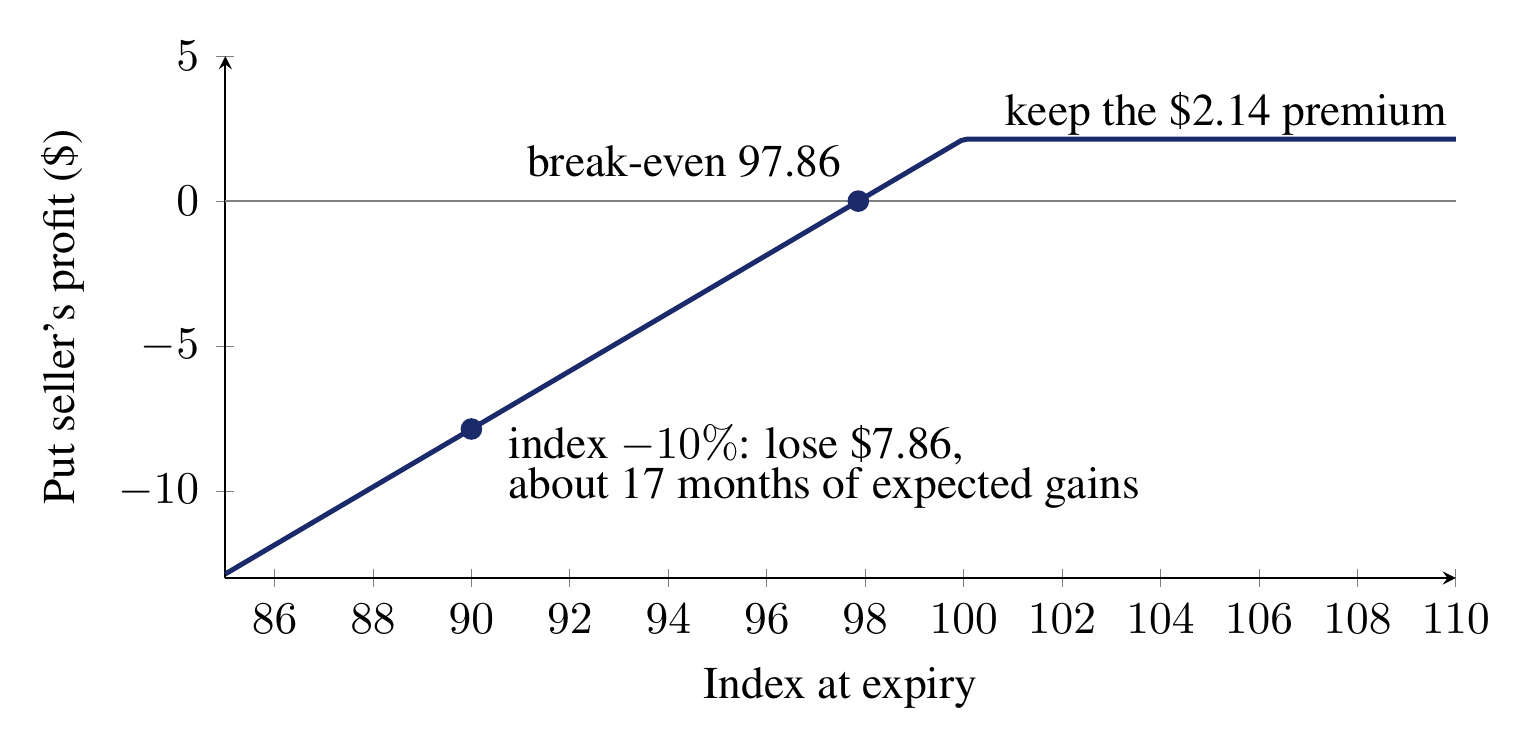
\includegraphics[width=0.85\linewidth]{images/fig14-1-short-put.png}
\caption{The put seller's profit at expiry in the worked example. Above the strike of 100 the seller keeps the \$2.14 premium; below the break-even of 97.86 the loss grows one for one with the fall. A 10\% fall costs \$7.86, about seventeen months of expected gains.}
\label{fig:14-put}
\end{figure}

\textbf{Further reading.} Hull, \emph{Options, Futures, and Other Derivatives} (option properties, put--call parity, Black--Scholes--Merton, the Greeks, volatility smiles, variance swaps); Natenberg, \emph{Option Volatility and Pricing}; Bodie, Kane and Marcus, \emph{Investments} (option strategies); Gatheral, \emph{The Volatility Surface}.

\section{How it works}
\label{sec:14-how}

\textbf{Why insurance might be overpriced.} Many investors hold stock portfolios they cannot easily sell and want protection against crashes. Pension funds, insurers and structured-product issuers buy index puts; market makers who sell them must hold capital against the risk and cannot fully hedge it. Bollen and Whaley (2004) and G\^arleanu, Pedersen and Poteshman (2009) showed that this net buying pressure raises option prices, especially for out-of-the-money puts. In equilibrium, sellers are paid for bearing a risk that bites in the worst states of the world, when investors' wealth is low and losses hurt most. A premium for that risk is not a free lunch. It is compensation, and it should be large precisely because the losses come at bad times.

\textbf{Ways to sell volatility.} The strategies differ in how much equity risk they carry alongside the volatility exposure.

\begin{center}
\small
\begin{tabularx}{0.9\linewidth}{@{}>{\raggedright\arraybackslash}p{0.19\linewidth}>{\raggedright\arraybackslash}X>{\raggedright\arraybackslash}X>{\raggedright\arraybackslash}X@{}}
\toprule
Strategy & Position & Equity exposure & Main risk \\
\midrule
Covered call (buy-write) & Own the index, sell a call & High (beta about 0.5--0.8) & Market falls; gains capped in rallies \\
Cash-secured put (put-write) & Hold bills, sell a put & High (same as covered call at the same strike) & Market falls \\
Short straddle & Sell a call and a put & Low on average, changes with the market & Large moves either way \\
Delta-hedged option & Sell an option, hedge its delta daily & Near zero & Realized volatility above implied \\
Short variance swap & Receive fixed variance, pay realized & Near zero, but crashes raise realized variance & Volatility spikes \\
\bottomrule
\end{tabularx}
\end{center}

The first two are what most retail and institutional ``option income'' products do. The last two isolate the variance risk premium itself. Comparing them is the heart of this chapter: if the covered call's return is mostly the equity premium earned with a beta of 0.6, it is not evidence that selling options pays.

\textbf{The payoff shape.} A covered call keeps the downside of the stock market but caps the upside at the strike plus the premium (Figure~\ref{fig:14-cc}). In calm or gently rising months it beats the market; in strong rallies it lags; in crashes it loses almost as much as the market, cushioned only by the premium. The return distribution is therefore \textbf{negatively skewed}. Most months bring small gains, and a few bring large losses.

\begin{figure}[htbp]
\centering
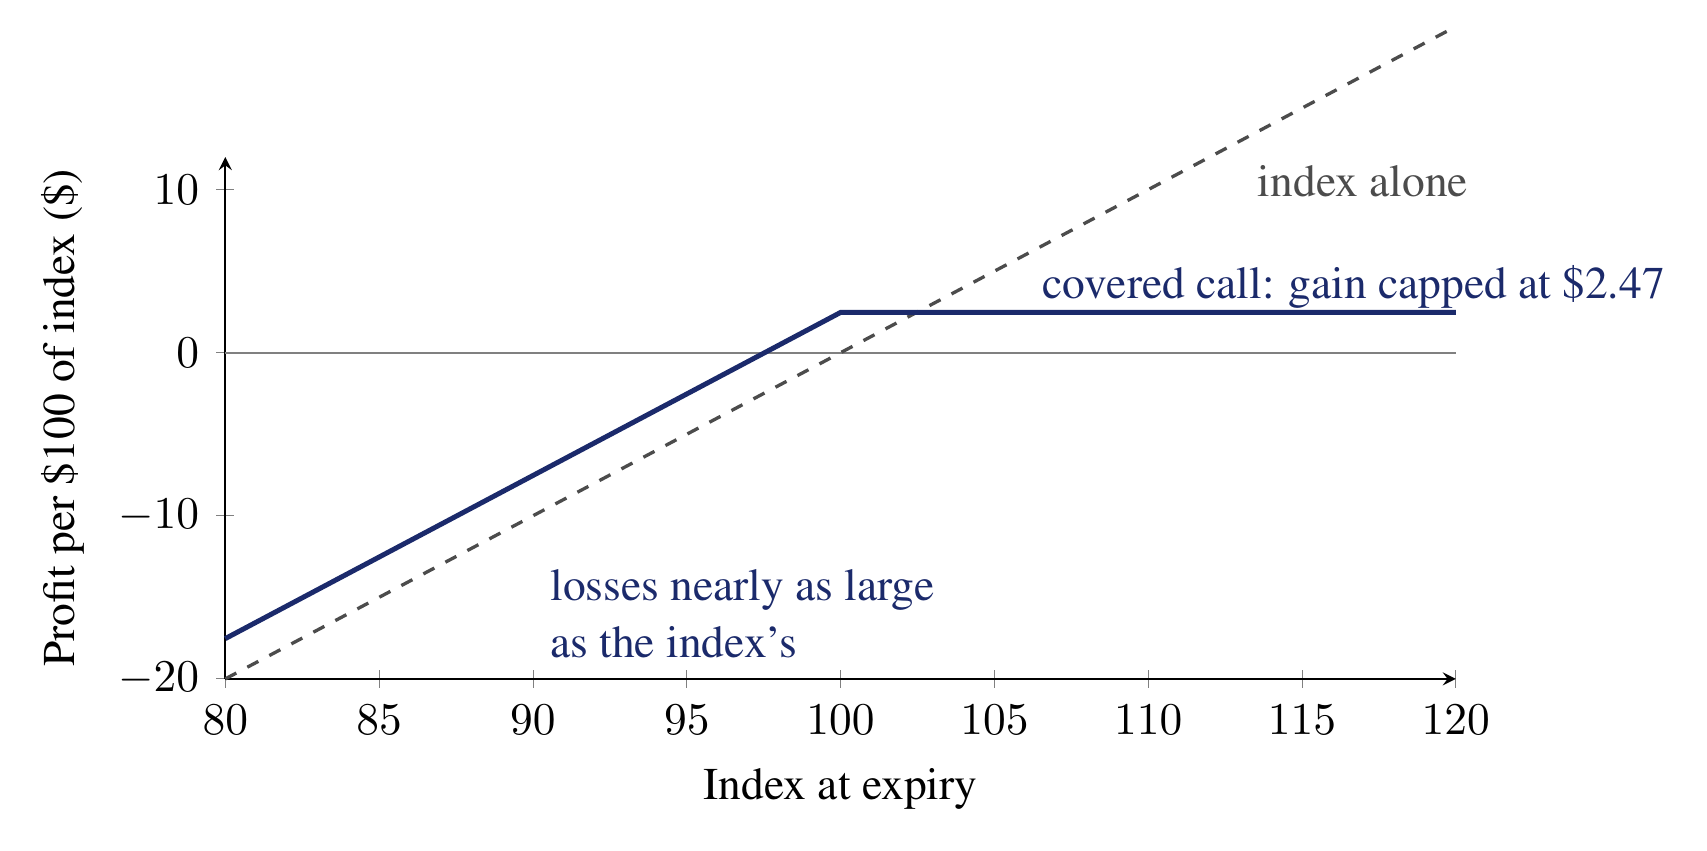
\includegraphics[width=0.85\linewidth]{images/fig14-2-covered-call.png}
\caption{A one-month at-the-money covered call against the index alone, using the worked example's prices. The call premium of \$2.47 caps the gain and cushions the loss by the same amount, so the covered call keeps almost all of the index's downside.}
\label{fig:14-cc}
\end{figure}

That shape creates a measurement problem. The Sharpe ratio uses only the mean and standard deviation, so it cannot see skewness. Selling out-of-the-money options can raise a portfolio's Sharpe ratio while making its tail much worse. Section~\ref{sec:14-measure} sets out measures that are harder to game.

\section{The claim}
\label{sec:14-claim}

\begin{callout}
\textbf{Claim.} Implied volatility exceeds the volatility that follows, on average, so option sellers earn a reliable premium. Strategies that sell index options, such as covered calls and put-writing, deliver better risk-adjusted returns than holding the index.
\end{callout}

The claim has two parts that can succeed or fail separately.

\begin{itemize}
  \item \textbf{The variance risk premium.} Implied variance is, on average, above the realized variance that follows. This is a statement about prices and can be tested directly by comparing the VIX with subsequent realized volatility.
  \item \textbf{The strategy premium.} Covered-call and put-writing strategies earn more than their risk justifies. This requires the variance premium to survive trading costs, early exercise and roll timing, and it requires an honest risk adjustment.
\end{itemize}

To test it we need to be precise on three points.

\begin{itemize}
  \item \textbf{What counts as risk.} A strategy with a beta of 0.5 should be compared with half the market plus half in bills, not with the whole market. Its negative skewness should be priced, not ignored.
  \item \textbf{What counts as reliable.} A premium that is positive in most months but wiped out in a few is reliable in one sense and not in another. We report both the share of months positive and the size of the worst losses.
  \item \textbf{What would count against it.} The variance risk premium fails if implied volatility is not significantly above realized volatility on average. The strategy claim fails if covered calls and put-writing earn no alpha after adjusting for beta, or if their advantage disappears once skewness is priced.
\end{itemize}

\section{The original evidence}
\label{sec:14-evidence}

\textbf{Option returns.} Coval and Shumway (2001) studied S\&P 500 index options and found that buying zero-beta, at-the-money \textbf{straddles} (a call and a put at the same strike) lost about 3\% a week on average. A straddle has little exposure to the direction of the market, so its losses point to a price for volatility itself. Bakshi and Kapadia (2003) found that delta-hedged option positions lost money on average, and attributed the losses to a negative market volatility risk premium: investors pay to be long volatility because volatility rises when markets fall.

\textbf{The variance risk premium.} Carr and Wu (2009) showed how to compute the variance swap rate from a portfolio of options, the method behind today's VIX, and used it to measure the premium directly for five stock indexes and 35 individual stocks. For the S\&P 500, implied variance was well above realized variance on average. Bollerslev, Tauchen and Zhou (2009) found that the size of the premium also predicts stock-market returns at a quarterly horizon, better than the price--earnings ratio or the default spread, consistent with its being a price of economic uncertainty.

\textbf{Covered calls and put-writing.} Cboe commissioned Robert Whaley to design the BuyWrite Index (BXM), which tracks an S\&P 500 portfolio that sells a one-month, near-the-money call each month. Whaley (2002) found that it had earned returns close to the S\&P 500's with substantially lower volatility. A later study for Cboe (Callan Associates 2006) reported that from June 1988 to August 2006 the BXM returned 11.77\% a year against 11.67\% for the S\&P 500, with a standard deviation of 9.29\% against 13.89\%. Cboe later added a PutWrite Index (PUT), which sells one-month at-the-money puts against Treasury-bill collateral. These results drew large inflows into option-income products.

\textbf{The skeptics.} Broadie, Chernov and Johannes (2009) argued that large average losses on index puts are not by themselves evidence of mispricing. Under standard models with jumps and reasonable risk premiums, put returns are expected to be very negative and very noisy, so short samples say little. Israelov and Nielsen (2015) decomposed covered-call returns into three exposures: the equity market, short volatility and an unintended equity reversal bet. Equity exposure drove most of the risk and return. The short-volatility component had a Sharpe ratio near 1.0 but contributed less than 10\% of the risk, and the reversal component added about a quarter of the risk with little return. A covered call, in other words, is mostly a stock-market position.

\section{Measuring option-strategy returns}
\label{sec:14-measure}

Option-selling strategies are the textbook case where the usual performance measures mislead. Four corrections matter.

\textbf{Adjust for beta.} A covered call with a beta of 0.6 should earn about 60\% of the equity premium without any volatility premium at all. The relevant comparison is a \textbf{beta-matched} portfolio, 60\% in the market and 40\% in bills, or equivalently the CAPM alpha (Chapter 12). A covered call that matches the market's return with two-thirds of its volatility may have earned no alpha.

\textbf{Look at both betas.} Selling options makes exposure asymmetric. The \textbf{down beta}, estimated in months when the market falls, is close to 1: the strategy takes most of the loss. The \textbf{up beta}, estimated in rising months, is much lower, because the call caps the gains. An investor who cares about losses more than gains should weigh the down beta.

\textbf{Price the skewness.} The Sharpe ratio ignores skewness, so a strategy can raise it by selling crash insurance. Goetzmann, Ingersoll, Spiegel and Welch (2007) showed that a manager can raise a portfolio's Sharpe ratio by selling out-of-the-money options, without any skill. They proposed a \textbf{manipulation-proof performance measure (MPPM)}:
\begin{equation}
  \Theta = \frac{1}{(1 - \rho)\,\Delta t}\,\ln\!\left\{\frac{1}{T}\sum_{t=1}^{T}\left[\frac{1 + r_t}{1 + r_{f,t}}\right]^{1-\rho}\right\}
  \label{eq:14-mppm}
\end{equation}
Here $T$ is the number of periods, $\Delta t$ the length of each period in years, and $r_t$ and $r_{f,t}$ the strategy's and the risk-free return. $\Theta$ is the certainty-equivalent excess return of an investor with constant relative risk aversion $\rho$. With $\rho = 3$, a typical value, a large negative month costs far more than a large positive month gains, so selling crash insurance cannot improve the score unless it really adds value.

\textbf{Respect the sample.} A strategy that loses heavily once a decade needs several decades of data to estimate its mean (Section~\ref{sec:03-se}). Broadie, Chernov and Johannes (2009) showed how noisy put returns are even over twenty years. A backtest that starts after 2009 and ends before 2020, for example, would miss both of the big losses of the period since 1990.

\section{Replication lab: the VIX, put-writing and covered calls since 1990}
\label{sec:14-lab}

\begin{callout}
\textbf{Lab 14 at a glance.} \emph{Claim on trial:} selling index options earns a reliable premium. \emph{Data:} daily market returns from the Kenneth French library and the VIX from FRED, which starts in 1990; both are free. Cboe's PUT and BXM index histories can be added for comparison. \emph{Code:} runs as a script (\texttt{python lab14.py}) or as a notebook with a prediction prompt before each step.
\end{callout}

\textbf{Part A, the variance risk premium.} At each month end, the VIX is compared with the market's realized volatility over the next 21 trading days. The lab reports the average gap in volatility points with a Newey--West $t$-statistic, the share of months in which implied exceeded realized, the median gap and the worst months (Figures 14.3 and 14.4).

\textbf{Part B, strategies.} The lab rebuilds two strategies from the data. Each month it sells a one-month option priced by Black--Scholes at the VIX and holds it to the next month end:

\begin{itemize}
  \item an \textbf{at-the-money put-write}, collateralized by bills like Cboe's PUT. By put--call parity this is also an at-the-money covered call, and the lab checks that the two returns are identical;
  \item a \textbf{covered call 2\% out of the money}, which keeps more of the market's upside.
\end{itemize}

Each is compared with the market on excess return, volatility, Sharpe ratio, skewness, worst month, drawdown, beta and CAPM alpha, over its own history and over a common period (Figure 14.5).

\textbf{Part C, stress tests.} Returns in crisis periods, the five worst market months, up and down betas, and the MPPM (Figure 14.6).

\textbf{Part D, equity versus volatility.} Each strategy's excess return is split into the part explained by beta and the alpha that remains. The lab compares it with the market scaled to the same beta, and with a pure short variance swap struck at VIX$^2$, sized to 10\% annual volatility (Figure 14.7).

The rebuilt strategies are deliberately simple, and that matters for interpretation. They price options at the VIX, which includes the premium on out-of-the-money puts and so usually exceeds at-the-money implied volatility. That overstates the premium a seller actually collects. They also ignore bid--ask spreads and roll at month ends rather than on Cboe's third-Friday schedule. The \texttt{-{}-iv-shift} option prices the options a few points below the VIX. Comparing the rebuilt series with Cboe's indices, which use traded prices, shows how much these simplifications matter.

\textbf{What the simulated run shows.} The simulation builds in a VIX 12\% above expected volatility. The lab finds the premium (implied above realized in 83\% of months), a put-write with a beta of about 0.5, strongly negative skewness and a down beta near 0.9 against an up beta near 0.15. The rebuilt put-write and covered call show positive alphas when options are priced at the inflated VIX. The Cboe-like series, priced 2 points lower, show none. These results confirm that the code works. They say nothing about real markets. Run the lab on the real data to reach your own verdict.

\section{Stress tests}
\label{sec:14-stress}

\textbf{Crashes.} The months that decide the verdict are few: October 1987, August 1998, September 2008 to February 2009, February and March 2020. In each, the market fell sharply, realized volatility jumped far above the implied volatility priced a month earlier, and option sellers lost most of what the market lost. A put-write cushions a crash only by one month's premium, typically 1--3\% of the strike. Figure 14.4 shows the pattern for the variance premium: many small positive months and a few large negative ones.

\textbf{Skewness.} On the Sharpe ratio, put-writing and covered calls often look better than the market, because they cut volatility more than they cut returns. On the MPPM with risk aversion 3, expect the advantage to shrink, because the measure prices the crash months. A strategy whose apparent edge vanishes once skewness is priced is being paid for crash risk, not earning alpha.

\textbf{Equity exposure.} Covered calls and put-writes have betas of roughly 0.5 to 0.7. Over a period when the equity premium was large, a beta of 0.6 alone earns most of their return. The lab's decomposition separates the two: if the alpha is small relative to the beta component, the strategy is mainly a stock investment with a different payoff shape.

\textbf{Timing of the sample.} After a crisis, implied volatility can stay high while realized volatility subsides, which makes the premium look rich; before a crisis, it can look rich until the crash arrives. A backtest that starts just after a crisis, or ends just before one, will flatter the strategy. Exercise 4 splits the sample at 2008.

\textbf{Implementation.} Real options have bid--ask spreads, and covered-call funds pay management fees. Israelov and Nielsen (2015) found that the strategy's equity-reversal exposure, created by mechanically resetting the strike each month, adds risk without return. These frictions are small per trade but large relative to a premium of a few percent a year.

\section{Verdict}
\label{sec:14-verdict}

\begin{callout}
\textbf{Verdict: survives for the variance risk premium; weakens for option-income strategies} (as of October 2026). Implied volatility has exceeded subsequent realized volatility on average, in most months, across decades and markets. That premium is real and is compensation for crash risk. But covered-call and put-writing strategies earn most of their return from equity exposure, carry negative skewness and lose most of what the market loses in crashes. Measured against a beta-matched portfolio and with skewness priced, their advantage is small.
\end{callout}

What survives:

\begin{itemize}
  \item \textbf{The variance risk premium.} Studies using the VIX, synthetic variance swaps and option returns agree that index option buyers pay more than realized volatility justifies on average (Coval and Shumway 2001; Bakshi and Kapadia 2003; Carr and Wu 2009). The premium has an economic explanation, demand for crash insurance, and predicts market returns (Bollerslev, Tauchen and Zhou 2009).
  \item \textbf{Lower volatility for covered calls.} Covered calls and put-writes have delivered market-like returns with lower volatility over long periods. For an investor who has to hold equities, that is a real benefit.
\end{itemize}

What weakens it:

\begin{itemize}
  \item \textbf{Most of the return is equity.} With betas of 0.5 to 0.7, the strategies earn most of the equity premium through their stock exposure. The short-volatility component is a small share of their risk (Israelov and Nielsen 2015).
  \item \textbf{The Sharpe ratio flatters them.} Negative skewness and down betas near 1 mean that measures accounting for the tail, such as the MPPM, show a smaller advantage than the Sharpe ratio does.
  \item \textbf{The premium is paid for crash risk.} A pure short-volatility position earns a high Sharpe ratio most of the time and suffers severe losses in volatility spikes. Whether that is attractive depends on whether the investor can survive the spikes.
\end{itemize}

The verdict on option-income strategies would move to \emph{survives} if their alpha against a beta-matched benchmark remained significant after skewness and costs over a full cycle of crises. It would move to \emph{fails} if, after accounting for beta, the premium were consistently eaten by costs and fees.

\section{What investors can use}
\label{sec:14-investors}

\textbf{What an option-income fund actually delivers.} Covered-call and put-writing funds advertise high distributions. Three facts help interpret them; Israelov and Nielsen (2014) discuss these and other common misconceptions about covered calls.

\begin{itemize}
  \item \textbf{Distributions are not yield.} The premium a fund collects and pays out comes with a cap on the fund's gains. In a strong market, the investor gives up upside in exchange for the income. The premium is not a dividend on top of the market return; part of it is the market return, converted into a different shape.
  \item \textbf{The fund is mostly an equity fund.} With a beta of around 0.5 to 0.7 and a down beta near 1, it will fall nearly as much as the market in a crash and rise much less in a rally. Compare it with a mix of an index fund and bills at the same beta, not with the index.
  \item \textbf{Look at the worst months, not the Sharpe ratio.} A smooth return history can hide a tail. Ask how the fund did in 2008 and in March 2020.
\end{itemize}

\textbf{Questions to ask a manager selling volatility:}

\begin{itemize}
  \item What is the strategy's beta, and its down beta? What would a beta-matched index position have returned?
  \item How far out of the money, and how short-dated, are the options sold? How is the strike reset?
  \item What is the largest loss the strategy could suffer in one day, and how was that figure derived?
  \item Is there leverage, or margin that could be called in a spike?
\end{itemize}

\begin{callout}
\textbf{What Failed: selling volatility on margin, February 2018.} LJM Partners ran funds that used margin to sell out-of-the-money puts and calls on S\&P 500 futures. For years the strategy produced steady returns. In February 2018, when volatility spiked, the LJM-managed funds lost more than 80\%, over \$1 billion, in two trading days. The same week, the VelocityShares inverse VIX note described in Chapter 11 lost 96\% in a day.

In 2021 the SEC charged LJM and two portfolio managers with misleading investors about the funds' risk management. According to the SEC, the firm had told investors it stress-tested for a worst-case daily loss of 20\% in its mutual fund, but that figure had been derived from a historical single-day loss of about 9\%, doubled and rounded up.

The episode illustrates this chapter's verdict in its sharpest form. The variance risk premium is real, and selling volatility earned it for years. But the premium is payment for exactly the kind of day that ended LJM. Leverage turned a strategy that should lose heavily in a spike into one that could not survive it.
\end{callout}

\section{Open questions}
\label{sec:14-open}

\begin{itemize}
  \item \textbf{Has the boom in short-dated options changed the premium?} Options expiring the same day (zero days to expiry, or 0DTE) made up over 61\% of S\&P 500 index option volume in May 2025, according to Cboe (Cboe Global Markets 2025). Do they change the price of one-month volatility, or the size of the variance premium?
  \item \textbf{How large is the premium net of costs for retail investors?} Covered-call ETFs on single stocks and indexes have grown rapidly. What do they deliver after fees, spreads and taxes, compared with a beta-matched index position?
  \item \textbf{Is the premium compensation or mispricing?} Rational models with crash risk explain much of it (Broadie, Chernov and Johannes 2009). Does demand pressure from hedgers add a mispricing on top?
  \item \textbf{Can the premium be harvested with less crash risk?} Delta-hedged positions, variance swaps with caps, or strategies that cut exposure when volatility rises all aim to keep the premium and avoid the tail. Do they survive out of sample?
\end{itemize}

\section*{Exercises}
\addcontentsline{toc}{section}{Exercises}

\subsection*{Conceptual (all readers)}

\begin{enumerate}
  \item The index is at 4,000, the risk-free rate is 5\%, and one-month implied volatility is 18\%. Price a one-month at-the-money call and put by Black--Scholes and check put--call parity.
  \item Use put--call parity to show that a covered call and a cash-secured put with the same strike and expiry have the same payoff. Why do Cboe's BXM and PUT indices nonetheless have different returns?
  \item A covered call has a beta of 0.6 and has returned 7\% a year when the market returned 9\% and bills 2\%. What is its CAPM alpha? What return would a beta-matched portfolio of the index and bills have earned?
\end{enumerate}

\subsection*{Lab extensions (technical readers)}

\begin{enumerate}
  \setcounter{enumi}{3}
  \item Part A: in what share of months did the VIX exceed realized volatility? Compute the average gap separately for months with VIX above and below 25. Where is the premium larger? Then split the sample at 2008: how different is the premium before and after?
  \item Part B: rerun with \texttt{-{}-iv-shift -2} and \texttt{-4}. How much of the rebuilt put-write's alpha survives? Compare with Cboe's PUT if you downloaded it.
  \item Part C: compute the MPPM with risk aversion 1, 3 and 6. At what risk aversion does put-writing stop beating the market?
  \item Part D: what share of each strategy's excess return comes from beta? Compare the skewness of the put-write with that of the beta-matched market.
  \item Part D: the pure short variance swap has a high Sharpe ratio. Find its worst month. How much leverage could an investor have used before that month would have wiped out the account?
  \item A retiree is offered an option-income fund paying an 8\% distribution. Using this chapter's evidence, write a one-page explanation of what the fund is likely to deliver and what could go wrong.
\end{enumerate}

\section*{References}
\addcontentsline{toc}{section}{References}

\begin{itemize}
  \item Bakshi, G. and Kapadia, N. (2003). Delta-Hedged Gains and the Negative Market Volatility Risk Premium. \emph{Review of Financial Studies} 16(2): 527--566.
  \item Black, F. and Scholes, M. (1973). The Pricing of Options and Corporate Liabilities. \emph{Journal of Political Economy} 81(3): 637--654.
  \item Bollen, N. P. B. and Whaley, R. E. (2004). Does Net Buying Pressure Affect the Shape of Implied Volatility Functions? \emph{Journal of Finance} 59(2): 711--753.
  \item Bollerslev, T., Tauchen, G. and Zhou, H. (2009). Expected Stock Returns and Variance Risk Premia. \emph{Review of Financial Studies} 22(11): 4463--4492.
  \item Broadie, M., Chernov, M. and Johannes, M. (2009). Understanding Index Option Returns. \emph{Review of Financial Studies} 22(11): 4493--4529.
  \item Callan Associates (2006). \emph{An Historical Evaluation of the CBOE S\&P 500 BuyWrite Index Strategy}. Chicago: Cboe.
  \item Carr, P. and Wu, L. (2009). Variance Risk Premiums. \emph{Review of Financial Studies} 22(3): 1311--1341.
  \item Cboe Global Markets (2025). SPX 0DTE Options Jump to 61\% Share on Retail Resurgence. \emph{Cboe Insights}, June 2.
  \item Coval, J. D. and Shumway, T. (2001). Expected Option Returns. \emph{Journal of Finance} 56(3): 983--1009.
  \item G\^arleanu, N., Pedersen, L. H. and Poteshman, A. M. (2009). Demand-Based Option Pricing. \emph{Review of Financial Studies} 22(10): 4259--4299.
  \item Goetzmann, W., Ingersoll, J., Spiegel, M. and Welch, I. (2007). Portfolio Performance Manipulation and Manipulation-Proof Performance Measures. \emph{Review of Financial Studies} 20(5): 1503--1546.
  \item Israelov, R. and Nielsen, L. N. (2014). Covered Call Strategies: One Fact and Eight Myths. \emph{Financial Analysts Journal} 70(6): 23--31.
  \item Israelov, R. and Nielsen, L. N. (2015). Covered Calls Uncovered. \emph{Financial Analysts Journal} 71(6): 44--57.
  \item Merton, R. C. (1973). Theory of Rational Option Pricing. \emph{Bell Journal of Economics and Management Science} 4(1): 141--183.
  \item U.S. Securities and Exchange Commission (2021). SEC Charges LJM Funds Management and Portfolio Managers (complaint), June 2021.
  \item Whaley, R. E. (2002). Return and Risk of CBOE Buy Write Monthly Index. \emph{Journal of Derivatives} 10(2): 35--42.
\end{itemize}

\textbf{Data:} Kenneth R. French Data Library, Fama/French 3 Factors [Daily]. Chicago Board Options Exchange, CBOE Volatility Index: VIX [VIXCLS], retrieved from FRED, Federal Reserve Bank of St.\ Louis. Optional: Cboe S\&P 500 PutWrite (PUT) and BuyWrite (BXM) indices.
